\section{狄拉克记号}

\begin{quotation}
``记号法看来更能深入事物的本质,它可以使我们用简洁精炼的方式来表达物理规律''\qquad 狄拉克
\end{quotation}

\begin{figure}[h]
\begin{center}
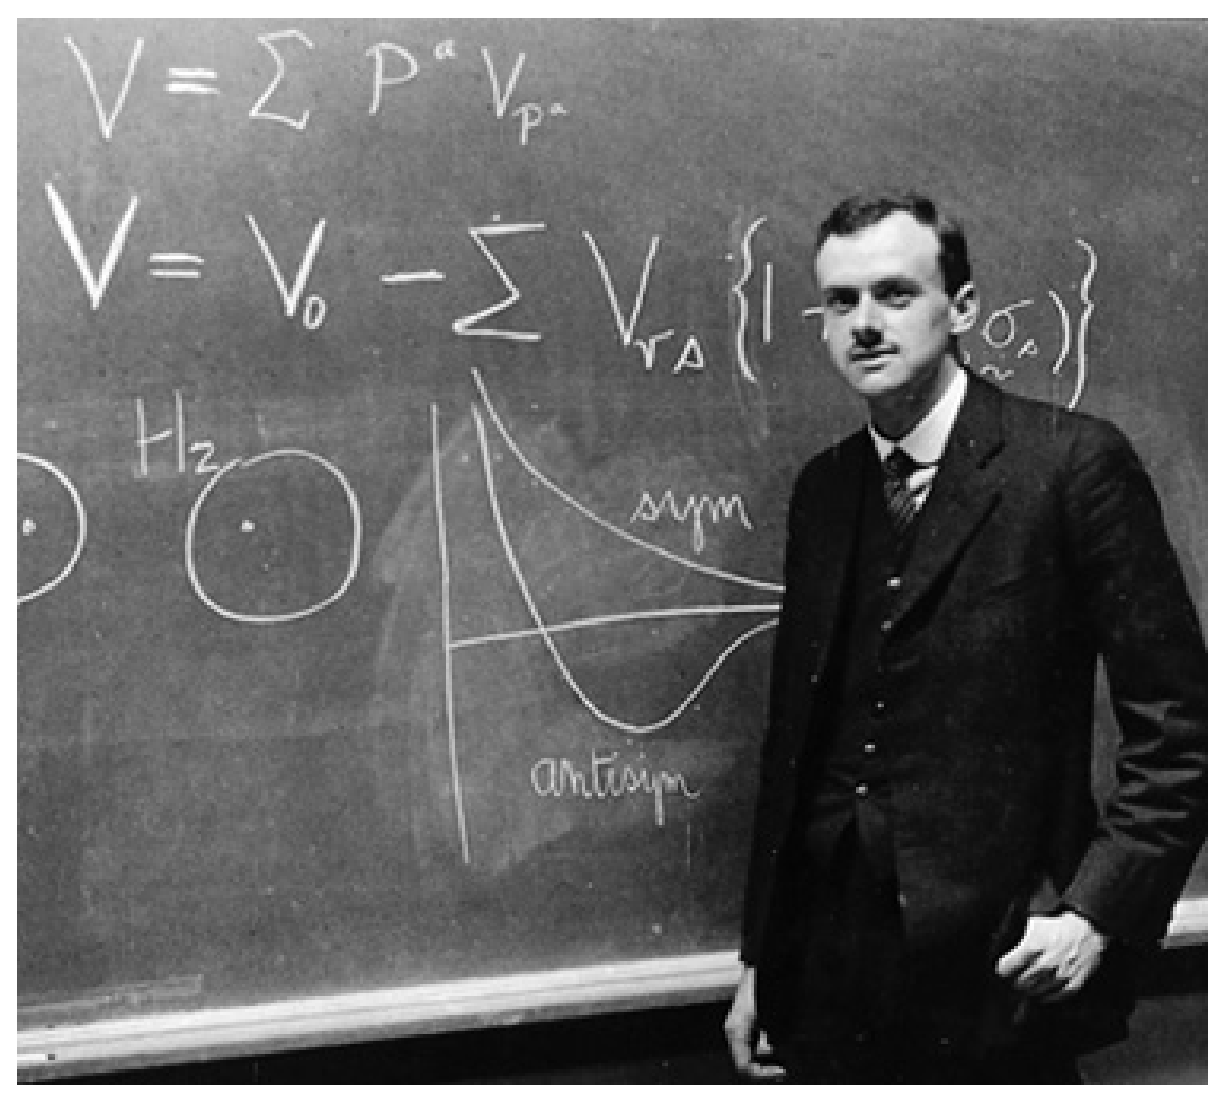
\includegraphics[clip,width=7cm]{Notation/dirac.ps}
\caption{狄拉克}
\end{center}
\end{figure}


在经典力学中, 物理规律与选择什么样的坐标系无关; 同样在量子力学中,
运动规律与选择的表象无关。狄拉克(Dirac)引入了一套不涉及具体表象的记号系统来表示波函数和力学量\footnote{不是$\psi(x)$或$\frac{\hbar}{i} \nabla$而是$\left| \psi \right\rangle  $和$\hat p$},称为狄拉克记号(Dirac Notation)。

选择适当的表象有利于量子力学问题的求解。一个好的记号系统同样也会有利于我们进行推演和计算。比如在经典力学中,莱布尼兹的微分和积分符号优于牛顿的符号系统被后人广泛采用;在量子力学中, 狄拉克的记号系统简单、易于进行理论推演、物理含义明显,因此被广泛使用。

\subsection{左矢、右矢和算符}

假设$\left| \alpha \right\rangle$是右矢空间\index{Ket space: 右矢空间}(Dirac Ket space, 任一希尔伯特空间都可充当右矢空间)中的一个矢量.
存在与右矢空间对应的对偶空间——左矢空间\index{Bra space: 左矢空间}(Dirac Bra space)——我们总可在左矢空间中中找到一个矢量与$\left| \alpha
\right\rangle$对应, 记作$\left\langle  \alpha \right|$, 反之亦然,
这种对应记作:



\begin{equation*}
\left\langle  \alpha \right|  \leftrightarrow \left| \alpha
\right\rangle
\end{equation*}

我们定义的这种对应还需要满足以下性质:

\begin{enumerate}
  \item $c^* \left\langle  \alpha \right| \leftrightarrow c \left| \alpha
\right\rangle $, 这里c是任意复数, 对复数c来说, 次序是不重要的, 即:
$c^* \left\langle  \alpha \right| = \left\langle  \alpha \right|
c^*$
  \item $c^*_1 \left\langle  \alpha \right| + c^*_2 \left\langle  \beta \right| \leftrightarrow  c_1 \left|
  \alpha \right\rangle + c_2 \leftrightarrow \left| \beta \right\rangle $

\end{enumerate}


从右矢空间中任取一个态矢量$\left| \alpha \right\rangle$,
从左矢空间任取另一个态矢量$\left\langle \beta \right|$,
我们可定义内积(inner product)运算, 映射为一个复数, $\left\langle
\beta | \alpha \right\rangle$, 并且满足:

\begin{equation*}
\left\langle \beta | \alpha \right\rangle = \left\langle \alpha |
\beta \right\rangle^*
\end{equation*}

我们定义的内积是正定的, 即: 自己和自己内积大于等于0.

\begin{equation*}
\left\langle \alpha | \alpha \right\rangle \geq 0
\end{equation*}

在此前提下, 我们可对非零态矢量归一化(Normalization),
得到所谓``归一化''的态矢量.

\begin{equation*}
\left\langle \alpha | \alpha \right\rangle =1
\end{equation*}



\subsubsection{厄米共轭}


在量子力学中, 物理系统运动状态由态矢量——如$\left| \alpha
\right\rangle$——表示, 算符A使一个态矢量$\left| \alpha
\right\rangle$映射为另一个态矢量$\left| \gamma \right\rangle$, 记作:

\begin{equation*}
\left| \gamma \right\rangle = A \left| \alpha \right\rangle
\end{equation*}

复数$c$和算符A是可以互相交换的:

\begin{equation*}
Ac \left| \alpha \right\rangle = c A \left| \alpha \right\rangle
\end{equation*}

$A \left| \alpha \right\rangle$是右矢空间中的一个矢量,
对应到左矢是$\left\langle \alpha \right| A^{\dagger}$,
$A^{\dagger}$是$A$的厄米共轭(Hermitian adjoint)\index{Hermitian adjoint: 厄米共轭},

\begin{equation*}
\left\langle \alpha \right| A^{\dagger} \leftrightarrow A \left|
\alpha \right\rangle
\end{equation*}

这意味着, 如果记$A \left| \alpha \right\rangle = \left| \gamma
\right\rangle$, 则$\left\langle \gamma \right| \leftrightarrow
\left| \gamma \right\rangle$, 这里$\left\langle \alpha \right|
A^{\dagger} = \left\langle \gamma \right|$, 即$\left\langle \alpha
\right| A^{\dagger}$是个左矢空间中的矢量.


如果我们计算内积$\left\langle \alpha | \gamma \right\rangle =
\left\langle \alpha | A | \alpha \right\rangle$, $\left\langle
\alpha | \gamma \right\rangle \leftrightarrow \left\langle \gamma |
\alpha \right\rangle = \left\langle \alpha \right| A^{\dagger}
\left| \alpha \right\rangle$, 所以:

\begin{equation*}
\left\langle \alpha \right| A^{\dagger} \left| \alpha \right\rangle
= \left\langle \alpha | \gamma \right\rangle^* = \left\langle \alpha
\right| A \left| \alpha \right\rangle^*
\end{equation*}



这里的$A$和$A^{\dagger}$未必相等, 如果$A = A^{\dagger}$,
则A是厄米算符. 由上式, 如果A是厄米算符,

\begin{equation*}
\left\langle \alpha \right| A \left| \alpha \right\rangle =
\left\langle \alpha \right| A \left| \alpha \right\rangle^*
\end{equation*}

一个复数的复共轭等于它自己, 意味着这个数, $\left\langle \alpha
\right| A \left| \alpha \right\rangle$, 是实数. 正是由于这个性质,
在量子力学中我们用厄米算符来表示物理量, 或力学量. 用$\left\langle
\alpha \right| A \left| \alpha \right\rangle$,
即``量子力学平均''来表示物理量的期望值(Expectation value).

对厄米算符, 求本征值问题(Eigen value problem),

\begin{equation*}
    A \left| a' \right\rangle = a' \left| a' \right\rangle
\end{equation*}

使得上式成立的$a'$叫本征值(Eigen value)\index{Eigen value: 本征值}, $\left| a' \right\rangle$是$a'$对应的本征矢(Eigen vector)\index{Eigen vector: 本征矢}.

我们可以证明如下性质: 如果A是厄米的话,

\begin{enumerate}
  \item A的本征值$a'$是实数;
  \item 对不同本征值如$a' \neq a''$, 它们对应的本征矢相互正交, 即: $\left\langle a' | a'' \right\rangle =0$.
\end{enumerate}

证: 为简单计, 假设本征值问题不存在简并, 即$a'$和$\left| a'
\right\rangle$是``一一对应''的.

首先: (1): $A \left| a' \right\rangle = a' \left| a' \right\rangle$,
$A \left| a'' \right\rangle = a'' \left| a'' \right\rangle$

把$A \left| a'' \right\rangle$对应到左矢空间, (2): $\left\langle a''
\right| A^{\dagger} = a''^* \left\langle a'' \right|$

对(1)式左乘$\left\langle a'' \right|$, 得到(3): $\left\langle a''
\right|A\left| a' \right\rangle = a' \left\langle a'' |a'
\right\rangle$

对(2)式右乘$\left| a' \right\rangle$, 得到(4): $\left\langle a''
\right| A^{\dagger} \left| a' \right\rangle = a''^* \left\langle a''
| a' \right\rangle$

(3)式-(4)式: $(a' - a''^*)\left\langle a'' | a' \right\rangle = 0$

假设$a' = a''$, $\left\langle a'' | a' \right\rangle \neq 0$, 则$a'
= a'*$, 即$a$是实数.

假设$a' \neq a''$, $a' - a'' \neq 0$, 那么: $\left\langle a'' | a'
\right\rangle = 0$

\subsubsection{运算的次序}

狄拉克记号中运算的次序很重要, 我们可能涉及到的有: 复数$c$, 算符$A,
B, ...$, 左矢$\left\langle {} \right|$, 右矢$\left| {}
\right\rangle$.

\begin{enumerate}
  \item 复数c可任意交换次序;
  \item 算符A, B, C,... 之间不能随意交换次序, 除非对易$AB = BA$;
  \item 内积: $\left\langle | \right\rangle$, ``乘出来''是个复数;
  \item 外积: $\left|  \right\rangle \left\langle  \right|$,
  ``乘出来''是个``算符'', 即$\left|  \right\rangle \left\langle
  \right|$可以把一个右矢映射为另一个右矢, 作为一个特例是投影算符\index{Project operator: 投影算符}:

\begin{equation*}
P_n = \left| n \right\rangle \left\langle n \right|
\end{equation*}

向``所有的方向''都作投影, 自然就得到单位算符\index{Unit operator: 单位算符}:

\begin{equation*}
\hat 1 = \sum\limits_{n} \left| n \right\rangle \left\langle n
\right|
\end{equation*}

\item 把算符A看作是``向右''运算的, 即都看作是对右矢作用的,  比较不容易出错. 比如, 把$\left\langle \alpha \right| A^{\dagger} \left| \alpha \right\rangle
  $看作: $\left\langle \alpha \right| \left( A^{\dagger} \left| \alpha
  \right\rangle \right)$,
  当然``$A^{\dagger}$''也可看作是``向左作用''的. 即先计算$\left| \gamma \right\rangle = A \left| \alpha
  \right\rangle$, 然后再把$\left| \gamma \right\rangle$对应到$\leftrightarrow \left\langle \gamma \right|$, 在此意义下, 我们把这个过程记作, 比如:
  $\left\langle A \alpha | \alpha \right\rangle$, 即: $\left\langle \alpha \right| \left( A^{\dagger} \left| \alpha
  \right\rangle \right) = \left\langle A \alpha | \alpha \right\rangle$.

  写成常见的波函数的形式, 就是: $\int dx (A\psi(x))^* \psi(x) = \int dx \psi^*(x) (A^{\dagger}
  \psi(x))$, 或:

\begin{equation*}
\int dx (A^{\dagger} \psi(x))^* \psi(x) = \int dx \psi^*(x) (A
\psi(x))
\end{equation*}

\end{enumerate}


\subsubsection{位置表象}

把单位算符$\hat 1$推广到连续谱, 比如$ x' $(位置), 有:

\begin{equation*}
\hat 1 = \int dx' \left| x' \right\rangle \left\langle x' \right|
\end{equation*}

把此单位算符作用于任意态矢$\left| \alpha \right\rangle$,

\begin{equation*}
\int dx' \left| x' \right\rangle \left\langle x' | \alpha
\right\rangle
\end{equation*}

这里的复数因子$\left\langle x' | \alpha
\right\rangle$就是波函数$\psi_{\alpha}(x')$.
发现``粒子''在$x'$的几率是$\left| \psi_{\alpha}(x') \right|^2$.

归一化条件: $\left\langle \alpha | \alpha \right\rangle =1$, 即:

\begin{equation*}
1 = \int dx' \left\langle \alpha | x' \right\rangle \left\langle x'
| \alpha \right\rangle = \int dx' \left| \psi_{\alpha}(x')\right|^2
\end{equation*}

\subsubsection{小结}

\begin{description}
\item[量子态] $\psi = \left| {} \right\rangle $表示右矢空间中的一个向量,$\psi ^ +   =
\left\langle {} \right|$表示左矢空间中的一个向量;

\index{bra: 左矢}

\index{ket: 右矢}

若要表示某个特定的量子态, 则应标上相应的记号; 如: $\left| \alpha
\right\rangle $表示某个态$\alpha$;$\left| p \right\rangle
$表示动量为$p$的本征态;$\left| n \right\rangle
$表示能量为$E_n$的本征态;$\left| {l,m} \right\rangle
$表示角动量$\left( {\widehat L^2 ,\widehat L_z }
\right)$的共同本征态; $\left| t \right\rangle $表示时刻$t$的量子态。
这里, 量子态的表示都未涉及具体的表象。


\item[内积] $\left\langle {\varphi }
 \mathrel{\left | {\vphantom {\varphi  \psi }}
 \right. \kern-\nulldelimiterspace}
 {\psi } \right\rangle  = \left\langle {\psi }
 \mathrel{\left | {\vphantom {\psi  \varphi }}
 \right. \kern-\nulldelimiterspace}
 {\varphi } \right\rangle ^* $, $\left| \varphi  \right\rangle ,\left| \psi  \right\rangle $是任意两个量子态;

\index{Orthonormalization: 正交归一化}

正交归一条件:$\left\langle {\lambda }
 \mathrel{\left | {\vphantom {\lambda  {\lambda '}}}
 \right. \kern-\nulldelimiterspace}
 {{\lambda '}} \right\rangle  = \delta \left( {\lambda  - \lambda '} \right)$(连续谱), $\left\langle {m}
 \mathrel{\left | {\vphantom {m n}}
 \right. \kern-\nulldelimiterspace}
 {n} \right\rangle  = \delta _{mn} $(分立谱)


\item[量子态在具体表象中的表示] 

假设量子态在$A$表象中, 基矢: $\left| n
\right\rangle $;$\left| \psi  \right\rangle  = \sum\limits_n {a_n \left| n \right\rangle } $,$a_n  = \left\langle {n}
 \mathrel{\left | {\vphantom {n \psi }}
 \right. \kern-\nulldelimiterspace}
 {\psi } \right\rangle $


所以: $\left| \psi  \right\rangle  = \sum\limits_n {\left\langle {n}
 \mathrel{\left | {\vphantom {n \psi }}
 \right. \kern-\nulldelimiterspace}
 {\psi } \right\rangle \left| n \right\rangle }  = \sum\limits_n {\left| n \right\rangle \left\langle {n}
 \mathrel{\left | {\vphantom {n \psi }}
 \right. \kern-\nulldelimiterspace}
 {\psi } \right\rangle } $

定义投影算符:$P_n  = \left| n \right\rangle \left\langle n \right|$,$P_n$的作用是求出态矢在$\left| n \right\rangle $方向的分量:

\index{Project operator: 投影算符}

$P_n \left| \psi  \right\rangle  = \left| n \right\rangle \left\langle n \right|\left. \psi  \right\rangle  = \left| n \right\rangle a_n  = a_n \left| n \right\rangle $

\index{Unit operator: 单位算符}

单位算符:

\begin{equation}
I \equiv \sum\limits_n {\left| n \right\rangle \left\langle n \right|} 
\end{equation}

对任何正交完备归一基矢$\{ \left| n \right\rangle \} $都满足;

\index{Completeness: 完备性}

连续谱情形:

\begin{equation}
I \equiv \int {\left| {x'} \right\rangle }
dx'\left\langle {x'} \right|
\end{equation}

任何一组正交归一完备本征函数都可用来构造$\delta$函数\footnote{参考曾谨言《量子力学 卷I》第729页}:

\index{Completeness: 完备性}

$\left\langle {x}
 \mathrel{\left | {\vphantom {x {x'}}}
 \right. \kern-\nulldelimiterspace}
 {{x'}} \right\rangle  = \sum\limits_n {\left\langle {x}
 \mathrel{\left | {\vphantom {x n}}
 \right. \kern-\nulldelimiterspace}
 {n} \right\rangle \left\langle {n}
 \mathrel{\left | {\vphantom {n {x'}}}
 \right. \kern-\nulldelimiterspace}
 {{x'}} \right\rangle }  = \delta \left( {x - x'} \right)$

例:

$\delta \left( {\varphi  - \varphi '} \right) = \frac{1}{{2\pi
}}\sum\limits_{m =  - \infty }^\infty  {\exp \left[ { - im\left(
{\varphi  - \varphi '} \right)} \right]} $

$\delta \left( {\cos \theta  - \cos \theta '} \right) =
\sum\limits_{l = 0}^\infty  {\frac{{2l + 1}}{2}P_l (\cos \theta
')P_l (\cos \theta )} $



\item[算符在具体表象中的表示] 态矢量在$A$表象中,基矢:$\left| n \right\rangle $

$\left| \varphi  \right\rangle  = \widehat F\left| \psi  \right\rangle $


$\left\langle {m}
 \mathrel{\left | {\vphantom {m \varphi }}
 \right. \kern-\nulldelimiterspace}
 {\varphi } \right\rangle  = \left\langle m \right|\widehat F\left| \psi  \right\rangle  = \sum\limits_n {\left\langle m \right|} \widehat F\left| n \right\rangle \left\langle {n}
 \mathrel{\left | {\vphantom {n \psi }}
 \right. \kern-\nulldelimiterspace}
 {\psi } \right\rangle $, 即:$b_m  = \sum\limits_n {F_{mn} a_n } $

矩阵元:$F_{mn}  = \left\langle m \right|\widehat F\left| n \right\rangle $


算符$\hat F$的本征方程:$\widehat F\left| \psi  \right\rangle  = \lambda \left| \psi  \right\rangle $

\index{Eigenequation: 本征方程}

$\left\langle m \right|\widehat F\left| \psi  \right\rangle  = \sum\limits_n {\left\langle m \right|\widehat F\left| n \right\rangle \left\langle n \right|\left. \psi  \right\rangle }  = \lambda \left\langle {m}
 \mathrel{\left | {\vphantom {m \psi }}
 \right. \kern-\nulldelimiterspace}
 {\psi } \right\rangle $


即: $\sum\limits_n {\left( {F_{mn}  - \lambda \delta _{mn} }
\right)a_n }  = 0$

薛定谔方程: $i\hbar \frac{\partial }{{\partial t}}\left| \psi
\right\rangle  = \widehat H\left| \psi  \right\rangle $

\index{Schrodinger equation: 薛定谔方程}

$i\hbar \frac{\partial }{{\partial t}}\left\langle {m}
 \mathrel{\left | {\vphantom {m \psi }}
 \right. \kern-\nulldelimiterspace}
 {\psi } \right\rangle  = \left\langle m \right|\widehat H\left| \psi  \right\rangle  = \sum\limits_n {\left\langle m \right|} \widehat H\left| n \right\rangle \left\langle {n}
 \mathrel{\left | {\vphantom {n \psi }}
 \right. \kern-\nulldelimiterspace}
 {\psi } \right\rangle $



即:$i\hbar \frac{\partial }{{\partial t}}a_m  = \sum\limits_n {H_{mn} a_n } $


力学量的平均值: $\overline F  = \left\langle \psi  \right|\widehat F\left| \psi  \right\rangle  = \sum\limits_{mn} {\left\langle \psi  \right|} \left. m \right\rangle \left\langle m \right|\widehat F\left| n \right\rangle \left\langle {n}
 \mathrel{\left | {\vphantom {n \psi }}
 \right. \kern-\nulldelimiterspace}
 {\psi } \right\rangle  = \sum\limits_{mn} {a_m^* F_{mn} a_n } $

   \end{description}


\subsection{表象变换}

\index{Change of representation: 表象变换}

对力学量$A$,有本征值问题:$A \left| a \right\rangle = a \left| a
\right\rangle$;正交归一本征矢的集合$\{ \left| a \right\rangle
\}$构成完备集,即:

\begin{equation*}
1 = \sum\limits_a {\left| a \right\rangle \left\langle a \right|} 
\end{equation*}

任一态矢$\left| \alpha \right\rangle$可表示为所有$\left| a
\right\rangle$的线性迭加:

\begin{equation*}
\left| \alpha  \right\rangle  = \sum\limits_a {\left| a
\right\rangle \left\langle {a}
 \mathrel{\left | {\vphantom {a \alpha }}
 \right. \kern-\nulldelimiterspace}
 {\alpha } \right\rangle } 
\end{equation*}

\index{Representation: 表象}

迭加系数为$c_a  = \left\langle {a}
 \mathrel{\left | {\vphantom {a \alpha }}
 \right. \kern-\nulldelimiterspace}
 {\alpha } \right\rangle $, 可用列向量$c_a$表示,我们也称$c_a$为$A$表象下的波函数。

现在取$B$表象,即对力学量$B$,也有本征值问题:$B \left| b
\right\rangle = b \left| b \right\rangle $,$\{ \left| b
\right\rangle \}$也构成正交归一完备集(Complete orthonormal set),

\index{Complete orthonormal set: 正交归一完备集}

\begin{equation*}
1 = \sum\limits_b {\left| b \right\rangle \left\langle b \right|} 
\end{equation*}

类似地, 任一态矢$\left| \alpha \right\rangle$可表示为所有$\left| b
\right\rangle$的线性迭加:

\begin{equation*}
\left| \alpha  \right\rangle  = \sum\limits_b {\left| b
\right\rangle \left\langle {b}
 \mathrel{\left | {\vphantom {b \alpha }}
 \right. \kern-\nulldelimiterspace}
 {\alpha } \right\rangle } 
\end{equation*}

迭加系数为$c_b  = \left\langle {b}
 \mathrel{\left | {\vphantom {b \alpha }}
 \right. \kern-\nulldelimiterspace}
 {\alpha } \right\rangle$, 可用列向量$c_b$表示。现在需要研究$A$(旧), $B$(新)表象间的变换关系。

\subsubsection{波函数}

$\left| \alpha  \right\rangle  = \sum\limits_i {\left| {b_i }
\right\rangle \left\langle {{b_i }}
 \mathrel{\left | {\vphantom {{b_i } \alpha }}
 \right. \kern-\nulldelimiterspace}
 {\alpha } \right\rangle }  = \sum\limits_{i,j} {\left| {b_i } \right\rangle \left\langle {{b_i }}
 \mathrel{\left | {\vphantom {{b_i } {a_j }}}
 \right. \kern-\nulldelimiterspace}
 {{a_j }} \right\rangle \left\langle {{a_j }}
 \mathrel{\left | {\vphantom {{a_j } \alpha }}
 \right. \kern-\nulldelimiterspace}
 {\alpha } \right\rangle } $

定义变换矩阵$S_{ij}  = \left\langle {{b_i }}
 \mathrel{\left | {\vphantom {{b_i } {a_j }}}
 \right. \kern-\nulldelimiterspace}
 {{a_j }} \right\rangle $, 取$\left| {b_i } \right\rangle  \buildrel\textstyle.\over= \left( {0,0,...,1,0,0,...} \right)^T $(其中$1$是在第$i$个位置), 这样可得到矩阵表示:

$ \left( {\begin{array}{*{20}c}
   {...}  \\
   {c_i (b)}  \\
   {...}  \\
\end{array}} \right) = \left( {\begin{array}{*{20}c}
   {...} & {...} & {...}  \\
   {...} & {S_{ij} } & {...}  \\
   {...} & {...} & {...}  \\
\end{array}} \right)\left( {\begin{array}{*{20}c}
   {...}  \\
   {c_j (a)}  \\
   {...}  \\
\end{array}} \right)
$,

简记作:$\chi (b) = S \chi (a)$,此即新旧表象下波函数的变换关系。


\subsubsection{基矢}

假设基矢间变换关系通过$U$算符联系起来,$\left| b_i \right\rangle = U
\left| a_i \right\rangle$,则:$\left\langle {b_i } \right| =
\left\langle {a_i } \right|U^\dag  $。

那么:$S_{ij}  = \left\langle {{b_i }}
 \mathrel{\left | {\vphantom {{b_i } {a_j }}}
 \right. \kern-\nulldelimiterspace}
 {{a_j }} \right\rangle  = \left\langle {a_i } \right|U^\dag  \left| {a_j } \right\rangle  = U_{ij}^\dag  $。

\index{Unitary matrix: 幺正矩阵}

可以证明$U$是幺正矩阵(unitary)。

\begin{equation*}
\left\langle {a_i }
\right|U^\dag  U\left| {a_j } \right\rangle  = \left\langle {{b_i }}
 \mathrel{\left | {\vphantom {{b_i } {b_j }}}
 \right. \kern-\nulldelimiterspace}
 {{b_j }} \right\rangle  = \delta _{ij}
\end{equation*}

类似地, $S$也是幺正矩阵。

\begin{equation*}
\left( {S^\dag  S} \right)_{ij}  = \sum\limits_k {S_{ik}^\dag  S_{kj} }  = \sum\limits_k {\left\langle {{a_i }}
 \mathrel{\left | {\vphantom {{a_i } {b_k }}}
 \right. \kern-\nulldelimiterspace}
 {{b_k }} \right\rangle \left\langle {{b_k }}
 \mathrel{\left | {\vphantom {{b_k } {a_j }}}
 \right. \kern-\nulldelimiterspace}
 {{a_j }} \right\rangle }  = \delta _{ij} 
\end{equation*}

为了与波函数变换关系比较, 假设:

\begin{equation*}
\left| {b_j } \right\rangle  =
U\left| {a_j } \right\rangle  = \sum\limits_i {\left| {a_i }
\right\rangle \left\langle {a_i } \right|U\left| {a_j }
\right\rangle }  = \sum\limits_i {U_{ij} \left| {a_i } \right\rangle
} 
\end{equation*}

这里: $U_{ij}  = \left\langle {a_i } \right|U\left| {a_j }
\right\rangle  = \left\langle {{a_i }}
 \mathrel{\left | {\vphantom {{a_i } {b_j }}}
 \right. \kern-\nulldelimiterspace}
 {{b_j }} \right\rangle  = S_{ij}^\dag  $,所以基矢间变换关系可写为:$\left| b \right\rangle = S^{\dagger}
\left| a \right\rangle$。


\subsubsection{力学量期望值}

在$A$(旧)表象下, 对波矢$\left| \alpha
\right\rangle$计算力学量$F$的期望值:

$\bar F_A  = \left\langle \alpha  \right|F\left| \alpha
\right\rangle _A  = \sum\limits_{ij} {\left\langle {\alpha }
 \mathrel{\left | {\vphantom {\alpha  {a_i }}}
 \right. \kern-\nulldelimiterspace}
 {{a_i }} \right\rangle \left\langle {a_i } \right|F\left| {a_j } \right\rangle \left\langle {{a_j }}
 \mathrel{\left | {\vphantom {{a_j } \alpha }}
 \right. \kern-\nulldelimiterspace}
 {\alpha } \right\rangle }  = \chi ^\dag  (a)F(a)\chi (a)$


在$B$(新)表象下, 对波矢$\left| \alpha
\right\rangle$计算力学量$F$的期望值:

$\bar F_B  = \left\langle \alpha  \right|F\left| \alpha
\right\rangle _B  = \sum\limits_{ij} {\left\langle {\alpha }
 \mathrel{\left | {\vphantom {\alpha  {b_i }}}
 \right. \kern-\nulldelimiterspace}
 {{b_i }} \right\rangle \left\langle {b_i } \right|F\left| {b_j } \right\rangle \left\langle {{b_j }}
 \mathrel{\left | {\vphantom {{b_j } \alpha }}
 \right. \kern-\nulldelimiterspace}
 {\alpha } \right\rangle }  = \chi ^\dag  (b)F(b)\chi (b)$

这里:$\left\langle {a_i } \right|F\left| {a_j } \right\rangle  =
\sum\limits_{k,l} {\left\langle {{a_i }}
 \mathrel{\left | {\vphantom {{a_i } {b_k }}}
 \right. \kern-\nulldelimiterspace}
 {{b_k }} \right\rangle \left\langle {b_k } \right|F\left| {b_l } \right\rangle \left\langle {{b_l }}
 \mathrel{\left | {\vphantom {{b_l } {a_j }}}
 \right. \kern-\nulldelimiterspace}
 {{a_j }} \right\rangle } $, 新旧表象下, 矩阵元变换关系为:

$F(a)_{ij}  = \sum\limits_{k,l} {S_{ik}^\dag  F(b)_{kl} S_{lj} }
$,简记为:$F(a) = S^{\dagger} F(b) S$。

\subsubsection{小结}

新旧表象通过一幺正矩阵$S_{ij}  = \left\langle {{b_i }}
 \mathrel{\left | {\vphantom {{b_i } {a_j }}}
 \right. \kern-\nulldelimiterspace}
 {{a_j }} \right\rangle $联系起来,

\begin{itemize}
  \item 基矢的变换关系:$\left| b \right\rangle = S^{\dagger} \left| a \right\rangle$
  \item 波函数的变换关系:$\chi (b) = S \chi (a)$
  \item 矩阵元的变换关系:$F(b) = S F(a) S^{\dagger}$
\end{itemize}


\subsubsection{例子:三维转动}

作为一个例子,
我们把表象变换想象为三维空间中的定点旋转变换。更具体一点,
我们考虑围绕$z$轴的定轴旋转$R_z(\theta)$,
即围绕$z$轴按右手螺旋方向转动$\theta$角度。这里涉及是三维笛卡尔坐标系的基矢$(\vec
i, \vec j, \vec k)$旋转, 还是三维笛卡尔坐标系中的矢量$\vec V =
\left( {x,y,z} \right)^T $旋转的问题。
假设采取基矢旋转的观点:旧坐标系($O-xyz$),新坐标系($O-x'y'z'$),

\begin{figure}[h]
\begin{center}
\includegraphics[clip,width=6cm]{Notation/rotationfixpoint.ps}
\caption{围绕$z$轴旋转$\theta$角度}
\end{center}
\end{figure}

矢量坐标间变换关系为:


$\left( \begin{array}{l}
 x \\
 y \\
 z \\
 \end{array} \right) = \left( {\begin{array}{*{20}c}
   {\cos \theta } & { - \sin \theta } & 0  \\
   {\sin \theta } & {\cos \theta } & 0  \\
   0 & 0 & 1  \\
\end{array}} \right)\left( \begin{array}{l}
 {x'} \\
 {y'} \\
 {z'} \\
 \end{array} \right)$

令:$R_z \left( \theta  \right) = \left( {\begin{array}{*{20}c}
   {\cos \theta } & { - \sin \theta } & 0  \\
   {\sin \theta } & {\cos \theta } & 0  \\
   0 & 0 & 1  \\
\end{array}} \right)$,

新旧坐标间变换关系为:$( \text Old ) = R ( \text New
)$,由于$R$是正交矩阵($R^T R =1$),所以:$( \text New ) = R^T (
\text Old )$

对基矢而言,存在变换关系:



$\vec i' = ( \vec i' \cdot \vec i ) \vec i + ( \vec i' \cdot \vec j
) \vec j + ( \vec i' \cdot \vec k ) \vec k = \left( \begin{array}{l}
 \cos \theta  \\
 \sin \theta  \\
 0 \\
 \end{array} \right) = R_z (\theta) \vec i$


$\vec j' = ( \vec j' \cdot \vec i ) \vec i + ( \vec j' \cdot \vec j
) \vec j + ( \vec j' \cdot \vec k ) \vec k = \left( \begin{array}{l}
  - \sin \theta  \\
 \cos \theta  \\
 0 \\
 \end{array} \right) = R_z (\theta) \vec j$


$\vec k' = ( \vec k' \cdot \vec i ) \vec i + ( \vec k' \cdot \vec j
) \vec j + ( \vec k' \cdot \vec k ) \vec k = \left( \begin{array}{l}
 0 \\
 0 \\
 1 \\
 \end{array} \right) = R_z
(\theta) \vec k$



这组关系相当于$\left| b \right\rangle  = U\left| a \right\rangle
$,即这里的$R$对应$S^{\dagger}$,但$R$的矩阵元是实数,即$R$是正交矩阵(Orthogonal
matrix)。所以,基矢间变换关系为:$( \text{New basis} ) = R (
\text{Old basis} )$ ,或$( \text{Old basis} ) = R^T ( \text{New
basis} )$。


\subsection{三种绘景}


考虑薛定谔方程:

\begin{equation*}
    i \hbar \partial_t \psi(x,t)=H \psi(x,t)
\end{equation*}

可以形式地解为:

\begin{equation*}
    \psi(x,t)=e^{-iHt/\hbar} \psi(x,0)
\end{equation*}


某力学量的期望值为:$\left< A \right> = \left< \psi(x,t) | A |
\psi(x,t)\right>$,
如果我们认为物理系统的动力学行为(随时间演化的行为)完全由$\psi(x,t)$决定,
算符$A$不含时间,就是薛定谔绘景(Schordinger
picture);反之动力学行为完全由算符$A(t)$描述,而$\psi(x)$不含时间则为海森堡绘景(Heisenberg
picture)。这一点, 可由以下等式看出来:

\index{Schordinger picture: 薛定谔绘景}

\index{Heisenberg picture: 海森堡绘景}

\begin{equation*}
    \left< A \right> = \left< \psi(x,t) | A | \psi(x,t)\right> = \left<
\psi(x,0) | e^{iHt/\hbar}Ae^{-iHt/\hbar} | \psi(x,0) \right>
\end{equation*}


左边是薛定谔绘景,右边为海森堡绘景,为了标记的方便,我们对其进行如下改写:


\begin{itemize}
  \item 薛定谔绘景: $\psi^S(x,t) = \psi(x,t)$,$A^S =
A$。
  \item 海森堡绘景: $\psi^H(x)=\psi(x,0)=\psi^S(x,0)$,$A^H(t) =
e^{iHt/\hbar}Ae^{-iHt/\hbar}=e^{iHt/\hbar}A^Se^{-iHt/\hbar}$。
\end{itemize}



容易证明,对海森堡绘景而言,动力学问题由关于算符的运动方程(Equation
of motion)给出:

\index{Equation of motion: 运动方程}

\begin{equation*}
    i\hbar \partial_t A^H =[A^H,H]
\end{equation*}


考虑:$H = H_0 +
H'$,即哈密顿由本征值问题已知的$H_0$和微扰$H'$两部分组成(为了公式的简略,以下我们约定$\hbar=1$)。
由于:


\begin{equation*}
    \left\langle A \right\rangle  = \left\langle {\psi (x,t)} \right|A\left| {\psi (x,t)} \right\rangle  = \left\langle {\psi (x,t)} \right|e^{ - iH_0 t} e^{iH_0 t} Ae^{ - iH_0 t} e^{iH_0 t} \left| {\psi (x,t)} \right\rangle
\end{equation*}


受此启发,定义相互作用绘景(Interaction picture)为\footnote{参考:
J. J. Sakurai, \textbf{Modern Quantum Mechanics}, pp318;}:


\index{Interaction picture: 相互作用绘景}

\begin{eqnarray*}
% \nonumber to remove numbering (before each equation)
  \psi^I(x,t) &=& e^{iH_0t}\psi(x,t) = e^{iH_0t}\psi^S(x,t)\\
  A^I(t) &=& e^{iH_0t}Ae^{-iH_0t} = e^{iH_0t}A^Se^{-iH_0t}
\end{eqnarray*}

容易证明,它们分别满足如下动力学关系(以下公式中恢复$\hbar$):

\begin{equation*}
    i\hbar \partial_t \psi^I (x,t) = H'_I \psi^I (x,t)
\end{equation*}

这里$H'_I = e^{iH_0t/\hbar} H' e^{-iH_0t/\hbar}$;


\begin{equation*}
  i\hbar \partial_t A^I = [A^I, H_0]
\end{equation*}

即$\psi^I$的动力学行为只与微扰$H'_I$有关,而$A^I$的动力学行为完全由$H_0$描述。


\subsection*{练习}

\begin{enumerate}

\item 对动量算符$\hat p$, 证明:

\begin{equation*}
\left\langle x' \right| \hat p \left| \alpha \right\rangle
=\frac{\hbar}{i} \frac{\partial }{\partial x'} \left\langle x' |
\alpha \right\rangle
\end{equation*}



证: 动量算符的本征矢$\left| p' \right\rangle$也是完备的, 因此有:

\begin{equation*}
\hat 1 = \int dp' \left| p' \right\rangle \left\langle p' \right|
\end{equation*}

在$\hat p$与$\alpha$间插入单位算符,

\begin{equation*}
\int dp' \left\langle x' \right| \hat p \left| p' \right\rangle
\left\langle p' | \alpha \right\rangle = \int dp' p' \left\langle x'
| p' \right\rangle \left\langle p' | \alpha \right\rangle
\end{equation*}

上式中的$\left\langle x' | p'
\right\rangle$就是位置表象下的动量本征函数, 对应本征值为$p'$,


\begin{equation*}
\left\langle x' | p' \right\rangle = \frac{1}{\sqrt {2\pi \hbar}}
e^{ip'x'/\hbar}
\end{equation*}

因此:

\begin{equation*}
p' \left\langle x' | p' \right\rangle = \frac{\hbar}{i}
\frac{\partial}{\partial x'} \left\langle x' | p' \right\rangle
\end{equation*}

因此:

\begin{equation*}
\int dp' p' \left\langle x' | p' \right\rangle \left\langle p' |
\alpha \right\rangle = \int dp' \frac{\hbar}{i}
\frac{\partial}{\partial x'} \left\langle x' | p' \right\rangle
\left\langle p' | \alpha \right\rangle
\end{equation*}

由于$x'$和$p'$是独立的变量,
因此上式中的积分运算和微分运算可以颠倒次序, 因此:


\begin{equation*}
\left\langle x' \right| \hat p \left| \alpha \right\rangle =
\frac{\hbar}{i} \frac{\partial}{\partial x'} \int dp' \left\langle
x' | p' \right\rangle \left\langle p' | \alpha \right\rangle =
\frac{\hbar}{i} \frac{\partial }{\partial x'} \left\langle x' |
\alpha \right\rangle
\end{equation*}

证毕.


\item 对于$\left( L^2, L_z \right)$的共同本征态$\left|l,m \right\rangle$, 证明: $\left\langle L_x \right\rangle = \left\langle L_y \right\rangle = 0$; $\left\langle L_x^2 \right\rangle = \left\langle L_y^2 \right\rangle $; 对$L_x, L_y$验证满足不确定关系.

证: (1)回忆: $[L_y, L_z] =i\hbar L_x$, 所以:

\begin{equation*}
L_x = \frac{1}{i\hbar}(L_y L_z-L_zL_y)
\end{equation*}


所以:

$\left\langle L_x \right\rangle = \frac{1}{i\hbar} \left\langle lm
\right| L_y L_z-L_zL_y \left| lm \right\rangle = \frac{m\hbar}{i
\hbar} \left\langle lm \right| L_y - L_y \left| lm \right\rangle =
0$

类似地: $\left\langle L_y \right\rangle = 0$

由升降算符(或阶梯算符, ladder operator)出发,

\begin{eqnarray*}
% \nonumber to remove numbering (before each equation)
  L^+ &=& L_x + i L_y \\
  L^- &=& L_x - i L_y
\end{eqnarray*}



$L_x = \frac{L^+ + L^-}{2}$, $L_y = \frac{L^+ - L^-}{2i}$, $L^{\pm}
\left|lm \right\rangle \to \left|l,m \pm 1 \right\rangle $,

因此: $\left\langle L_x \right\rangle = \left\langle L_y
\right\rangle = 0$.

(2)$L_x^2 = \frac{1}{4}\left((L^+)^2 + (L^-)^2 + L^+ L^- + L^-
L^+\right)$,

$\left\langle L_x^2 \right\rangle = 0 + 0 + \frac{1}{4} \left\langle
L^+ L^- + L^- L^+ \right\rangle$



$L_y^2 = - \frac{1}{4}\left((L^+)^2 + (L^-)^2 - L^+ L^- - L^-
L^+\right)$

$\left\langle L_y^2 \right\rangle = 0 + 0 + \frac{1}{4} \left\langle
L^+ L^- + L^- L^+ \right\rangle$

因此: $\left\langle L_x^2 \right\rangle = \left\langle L_y^2
\right\rangle$

又由于: $ \left\langle L_z^2 \right\rangle = m^2 \hbar^2 $, $
\left\langle L^2 \right\rangle =l(l+1)\hbar^2 $, 所以:

\begin{equation*}
\left\langle L_x^2 \right\rangle = \left\langle L_y^2 \right\rangle
= \frac{(l(l+1)-m^2)\hbar^2}{2}
\end{equation*}


(3)考虑到:

$ \overline {( L_x - \overline {L_x} )^2} = \overline {L_x^2 +
(\overline {L_x})^2 - 2 L_x \overline {L_x}} = \overline{L_x^2} -
(\overline {L_x})^2 $

定义角动量的不确定:

\begin{equation*}
\Delta L_x = \sqrt {\overline{L_x^2} - (\overline {L_x})^2} = \hbar
\sqrt{\frac{l(l+1)-m^2}{2}}
\end{equation*}

类似地: $\Delta L_y = \hbar \sqrt{\frac{l(l+1)-m^2}{2}} $,

所以:

\begin{equation*}
\Delta L_x \Delta L_y = \frac{\hbar^2}{2} (l(l+1)-m^2)
\end{equation*}

由于$L_x, L_y$不对易, $[L_x, L_y]=i\hbar L_z$,
应满足如下不确定关系(uncertainty relation),

\begin{equation*}
\Delta L_x \Delta L_y \geq \frac{1}{2} \left| \overline{[L_x, L_y] }
\right| = \frac{m\hbar^2}{2}
\end{equation*}

当$m=\pm l$时, 左侧(L.H.S, Left hand side)存在最小值:
$\frac{l\hbar^2}{2}$, 由于$m= 0,\pm 1, \pm 2, ..., \pm l$,
左侧(L.H.S.) $\geq$ 右侧(R.H.S) 成立.

\item 对升降算符$L^{\pm} = L_x \pm i L_y$, 证明:

\begin{equation*}
L^{\pm} \left| lm \right\rangle = \hbar \sqrt{(l \mp m)(l \pm m +1)
} \left|l, m \pm 1 \right\rangle
\end{equation*}

证: 定义: $\left| \gamma \right\rangle = L^+ \left| lm
\right\rangle$, 对应到左矢空间, $\left\langle \gamma \right| =
\left\langle lm  \right| L^-$,

因此:

\begin{equation*}
\left\langle \gamma | \gamma \right\rangle = \left\langle lm \right|
L^- L^+ \left| lm \right\rangle
\end{equation*}

上式中的$L^- L^+$展开是:

\begin{equation*}
(L_x-iL_y) (L_x + i L_y) = L_x^2 + L_y^2 +i [L_x, L_y] = L^2 - L_z^2
- \hbar L_z
\end{equation*}

因此:

\begin{equation*}
\left\langle \gamma | \gamma \right\rangle = \left\langle L^2 -
L_z^2 - \hbar L_z \right\rangle = l(l+1)\hbar^2 - m^2\hbar^2 -m
\hbar^2
\end{equation*}

上式化简可得:

\begin{equation*}
\left\langle \gamma | \gamma \right\rangle =  (l - m)(l+m+1)\hbar^2
\end{equation*}

即: $L^{\pm} \left| lm \right\rangle = \hbar \sqrt{(l \mp m)(l \pm m
+1) } \left|l, m \pm 1 \right\rangle$, 的``upper sign'',
即$L^+$得证, 类似可证``lower sign'', $L^-$部分.


\item 轨道角动量量子数$l=1$, 在$L^2, L_z$共同表象下, 求: 算符$L_x, L_y, L_z, L^{\pm}$的矩阵表示; 求$L_x$的本征值及对应归一化本征矢.

解:
对$l=1$,$m=1,0,-1$。将$L^2$和$L_z$的共同本征态分别表示为三维列向量的基矢:

$\left|1,1 \right\rangle=\left( {\begin{array}{*{20}c}
   1  \\
   0  \\
   0  \\
 \end{array} } \right)$,$\left|1,0 \right\rangle =\left( {\begin{array}{*{20}c}
   0  \\
   1  \\
   0  \\
 \end{array} } \right)$,$\left|1,-1 \right\rangle =\left( {\begin{array}{*{20}c}
   0  \\
   0  \\
   1  \\
 \end{array} } \right)$

$L_z$的矩阵表示:$\left\langle \alpha  \right|L_z \left| \beta
\right\rangle  = \left( {\begin{array}{*{20}c}
   \hbar  & 0 & 0  \\
   0 & 0 & 0  \\
   0 & 0 & { - \hbar }  \\
\end{array}} \right)$;满足$L_z \left| l,m \right> = m \hbar
\left| l,m \right>$。

现在来计算$L^+$的矩阵元,考虑:$L^+ \left|1,-1 \right> = \sqrt{2}
\hbar \left|1,0 \right>$,$L^+ \left|1,0 \right> = \sqrt{2} \hbar
\left|1,1 \right>$

得到:

$\left\langle \alpha  \right|L^ +  \left| \beta  \right\rangle  =
\left( {\begin{array}{*{20}c}
   0 & {\sqrt 2 \hbar } & 0  \\
   0 & 0 & {\sqrt 2 \hbar }  \\
   0 & 0 & 0  \\
\end{array}} \right)$

由于:$(L^+)^\dagger = L^-$,得到:

$\left\langle \alpha  \right|L^ -  \left| \beta  \right\rangle  =
\left( {\begin{array}{*{20}c}
   0 & 0 & 0  \\
   {\sqrt 2 \hbar } & 0 & 0  \\
   0 & {\sqrt 2 \hbar } & 0  \\
\end{array}} \right)$

利用$L_x = \frac{L^+ + L^-}{2}$,可得到$L_x$的矩阵元:


$\left( {L_x } \right)_{\alpha \beta }  = \left(
{\begin{array}{*{20}c}
   0 & {\frac{\hbar }{{\sqrt 2 }}} & 0  \\
   {\frac{\hbar }{{\sqrt 2 }}} & 0 & {\frac{\hbar }{{\sqrt 2 }}}  \\
   0 & {\frac{\hbar }{{\sqrt 2 }}} & 0  \\
\end{array}} \right)$,

同理可得到$L_y$的矩阵元。

现在来研究本征值问题:$L_x \left( {\begin{array}{*{20}c}
   a  \\
   b  \\
   c  \\
\end{array}} \right) = \lambda \hbar \left( {\begin{array}{*{20}c}
   a  \\
   b  \\
   c  \\
\end{array}} \right)$


根据久期方程:$\det (L_x - \lambda \text{I}) =0$,解出:$\lambda^3 =
\lambda$,即:$\lambda =0, \pm 1$


把$\lambda =1$代回本征方程,解出:$\chi _1  = \left(
{\begin{array}{*{20}c}
   {\frac{1}{2}}  \\
   {\frac{{\sqrt 2 }}{2}}  \\
   {\frac{1}{2}}  \\
\end{array}} \right)$,


即:$\left|l=1,l_x=1 \right> = \frac{1}{2}\left|1,1 \right>+
\frac{\sqrt 2}{2} \left|1,0 \right> +\frac{1}{2}\left|1,-1 \right>$


把$\lambda =0$代回本征方程,解出:$\chi _0  = \frac{1}{{\sqrt 2
}}\left( {\begin{array}{*{20}c}
   1  \\
   0  \\
   { - 1}  \\
\end{array}} \right)$,

即:$\left|l=1,l_x=0 \right> = \frac{\sqrt 2}{2}\left|1,1 \right> -
\frac{\sqrt 2}{2}\left|1,-1 \right>$


把$\lambda = -1$代回本征方程,解出:$\chi _{ - 1}  = \left(
{\begin{array}{*{20}c}
   {\frac{1}{2}}  \\
   { - \frac{{\sqrt 2 }}{2}}  \\
   {\frac{1}{2}}  \\
\end{array}} \right)$,

即:$\left|l=1,l_x=-1 \right> = \frac{1}{2}\left|1,1 \right> -
\frac{\sqrt 2}{2} \left|1,0 \right> +\frac{1}{2}\left|1,-1 \right>$


同样也可以用$\chi_1$,$\chi_0$,$\chi_{-1}$来表示$\left|
1,1\right>$,$\left| 1,0\right>$,$\left| 1,-1\right>$:

$\left| 1,1 \right>=\frac{1}{2}\chi_1 + \frac{\sqrt 2}{2} \chi_0 +
\frac{1}{2}\chi_{-1}$

$\left| 1,0 \right>=\frac{\sqrt 2}{2}\chi_1 - \frac{\sqrt
2}{2}\chi_{-1}$

$\left| 1,-1 \right>=\frac{1}{2}\chi_1 - \frac{\sqrt 2}{2} \chi_0 +
\frac{1}{2}\chi_{-1}$

这意味着,比如对$\left| 11
\right>$测量$L_x$,其可能取值为$\hbar$,$0$,$-\hbar$;概率为:$\frac{1}{4}$,$\frac{1}{2}$和$\frac{1}{4}$。


\item 对$L^2, L_z$的共同本征态$Y_{10}$, 求$L_x$的可能测量值及相应概率.

解: $L_x$的可能测量值是$\hbar, 0 , -\hbar$, 相应概率分别是: $w_1,
w_0, w_{-1}$.

由: $\left\langle L_x \right\rangle = w_1 \hbar + 0 - w_{-1}\hbar  =
0$, 可得: $w_{1} = w_{-1}$.

再者: $\left\langle L_x^2 \right\rangle  = (w_1 + w_{-1})\hbar^2 =
\hbar^2$, 可知: $w_1=w_{-1} = 50$\%, $w_0 = 0$.


讨论: 假设是对$Y_{11}$进行测量, $L_x$的可能测量值是$\hbar, 0 ,
-\hbar$, 相应概率分别是: $w_+, w_0, w_-$.

由: $\left\langle L_x \right\rangle = w_+ \hbar + 0 - w_-\hbar  =
0$, 可得: $w_+ = w_-$

再者: $\left\langle L_x^2 \right\rangle  = (w_+ + w_-)\hbar^2 =
\frac{\hbar^2}{2}$, 可知: $w_+=w_- = 25$\%, $w_0 = 50$\%.



\item 在位置表象下, 求: 位置算符的矩阵元 $\left\langle x' \right| \hat x \left| x'' \right\rangle $, 动量算符的矩阵元$\left\langle x' \right| \hat p \left| x'' \right\rangle $.


解: (1)在位置表象下, $\hat x \left| x' \right\rangle = x' \left| x'
\right\rangle$, $\left\langle x' | x'' \right\rangle =
delta(x'-x'')$, 因此:


\begin{equation*}
\left\langle x' \right| \hat x \left| x'' \right\rangle = x''
\delta(x'-x'')
\end{equation*}

即: 位置算符的矩阵元在位置表象下是``对角型''的.

(2) $\left\langle x' \right| \hat p \left| x'' \right\rangle = \int
dp' \left\langle x' \right| \hat p \left| p' \right\rangle
\left\langle p' | x'' \right\rangle = \int dp' p' \left\langle x' |
p' \right\rangle \left\langle p' | x'' \right\rangle $

这里:

\begin{equation*}
\left\langle x' | p' \right\rangle = \frac{1}{\sqrt{2 \pi
\hbar}}e^{ip'x'/\hbar}
\end{equation*}

$\left\langle x' | p' \right\rangle$的物理含义即: 位置表象下,
动量$p'$的平面波.

利用:

\begin{equation*}
p' \left\langle x' | p' \right\rangle =
\frac{\hbar}{i}\frac{\partial }{\partial x'} \left\langle x' | p'
\right\rangle
\end{equation*}

则:

\begin{equation*}
\left\langle x' \right| \hat p \left| x'' \right\rangle = \int dp'
\frac{\hbar}{i}\frac{\partial }{\partial x'} \left\langle x' | p'
\right\rangle \left\langle p' | x'' \right\rangle
\end{equation*}

由于$x', p'$是两个独立的变量, 因此$\int
dp'$和$\frac{\partial}{\partial p'}$可交换次序.

\begin{equation*}
\left\langle x' \right| \hat p \left| x'' \right\rangle =
\frac{\hbar}{i}\frac{\partial }{\partial x'} \int dp' \left\langle
x' | p' \right\rangle \left\langle p' | x'' \right\rangle =
\frac{\hbar}{i}\frac{\partial }{\partial x'} \left\langle x' | x''
\right\rangle
\end{equation*}

注意这里$\delta$函数本身是偶函数, 但一求导, $\delta'$就是奇函数了,
因此上式中$x'$和$x''$的位置不能互换.



\end{enumerate}
